\documentclass{article}
\usepackage[pdftex]{graphicx}
\setlength{\textheight}{9.0in}
\setlength{\textwidth}{6.0in}
\setlength{\oddsidemargin}{0pt}
\setlength{\topmargin}{-0.5in}
\begin{document}

\title{Stimulus latency bug}
\author{Bruno A. Olshausen}
\maketitle

\noindent
{\bf\large Problem}
\vspace{0.1in}

Charlie and I discovered a bug in the stimulus presentation/data
acquisition system, which appears to be due to hardware failure on
ControlC.  We found the error by running some sparse noise test trials
in which the data acquisition was triggered off of ControlC.  We found
that ControlC's trigger to initiate data acquisition was not
synchronized with PresenterC's vertical sync signal (nor PresenterC's
`start' signal), so the actual beginning of stimulus presentation was
at some random interval (within a refresh cycle) after the initiation
of data acquisition.  We also noticed that the first trial within a
session is usually delayed by two or three vertical syncs from the
start of ControlC's trigger, whereas the remaining trials usually
begin stimulus presentation upon the first vertical sync after
ControlC's trigger.

Another set of bugs that were discovered at the same time are that
\begin{enumerate}
\item Timing information is not being written to the {\tt .INI} file
for sparse noise trials.  We believe that most of these trials were
run with a 1 ms stimulus latency, 1998 ms stimulus duration, and 1 ms
post-stimulus duration.  In the future, Presenter needs to be fixed to
write out timing information for {\em all} trials.

\item The refresh rate on PresenterC is not 85 Hz but rather 85.1 Hz.
Evidently no one bothered to actually measure this, so it was assumed
to be the value reported by the hardware, which is rounded off to the
nearest integer.  It is recommended that in the future the vertical
sync signal be acquired along with neural data.  This way, we will be
able to verify that PresenterC and ControllerC are synchronized, and
if there is any deviation or drift in PresenterC's vertical sync, we
will be able to correct for it.
\end{enumerate}

\vspace{0.25in}
\noindent
{\bf\large Possible workaround}
\vspace{0.1in}

There appears to be a simple fix for the variable stimulus latency
problem.  We noticed that for trials subsequent to the first within a
session, the distance between PresenterC's `start' and `stop' triggers
is always the same.  For example, for a 1998 ms stimulus duration, we
find that the distance between the two pulses is always 2021 ms.  The
situation is as follows:
\[
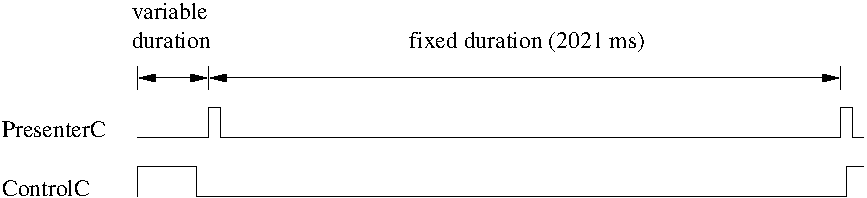
\includegraphics[width=6.0in]{latency_fig.pdf}
\]

The 2021 ms duration can be reconciled by assuming that PresenterC
waits until it is {\em over} the desired stimulus duration by an
integer number of frames before commanding a halt to data acquisition.
Once it decides to halt data acquisition, it actually does so on the
next refresh.  Since there are three refreshes per frame and 85.1
refreshes per second, we have
\begin{eqnarray}
\mbox{\rm \# of frames presented} & = & 
  \mbox{\rm ceil}\left(\frac{\mbox{\rm 1.998 sec.}}
			    {\mbox{(3 refreshes/frame)}/
			    \mbox{(85.1 refreshes/sec)}}\right) \\
 & = & 57 
\end{eqnarray}
where `ceil' means ``round up to nearest integer.''  Thus, the actual
stimulus duration is
\begin{equation}
\mbox{\rm 57 frames} \times 
  \mbox{\rm (3 refreshes/frame)}/\mbox{\rm (85.1 refreshes/sec)} +
  \mbox{\rm (1 refresh)}/\mbox{\rm (85.1 refreshes/sec)}  =  2.021\;\sec
\nonumber
\end{equation}

If our assumption is correct, we can re-align the data with the
stimulus by simply calculating the amount by which the data file
exceeds 2.021 sec (or whatever number is appropriate for the commanded
stimulus duration), and chop off the excess from the {\em beginning}
of the file.  Note however that this is a valid solution only for
trials subsequent to the first trial within a session.  For reasons
which we still do not understand, the first trials within a session do
not follow the above trend.

I have written two matlab functions for realigning the data.  The
first, called {\tt infer\_latency}, calculates the excess time for
each data file.  The second, {\tt shift\_spikes}, subtracts this
excess time from the spike times in the session structure generated by
{\tt GenerateSessionSpikeTrains}.  The raw data files are being left
alone for now.  Note that these routines are only applicable for data
collected before 9/01.  Data collected after this should be correctly
synced.

\end{document}

